\documentclass[11pt]{article}

\usepackage{fullpage}
\usepackage{graphicx}

\addtolength{\topmargin}{-0.6in}
\addtolength{\textheight}{1in}

\begin{document}

\title{Webapps Group Project: Project Technology Report}
\author{Group 21: Kam Chiu, Ho Law, Jiranart Vacheesuthum, Vasin Wongrassamee}

\maketitle

\section{Backend}
\begin{itemize}
\item Django python framework
\begin{itemize}
\item A language that all team members know
\item Robust
\item Does most heavy-lifting jobs 
\end{itemize}
\item Sqlite3 database
\begin{itemize}
\item lightweight
\item easy to use
\item we will soon switch to Postgresql database for better robustness
\end{itemize}
\end{itemize}
\begin{itemize}
\item django channels with in-memory channel layer 
\begin{itemize}
\item provides web-socket support
\item low latency and guaranteed delivery
\item works transparently with django
\end{itemize}
\end{itemize}

\section{Frontend}
\begin{itemize}
\item Yeoman development tools (yo, gulp, bower)
\begin{itemize}
\item modular architecture, comes with TDD enviroment
\item well-organised, easily managed or updates
\item easily scalable 
\end{itemize}
\end{itemize}


\begin{figure}[h]
\begin{minipage}{.5\textwidth}
  \centering
  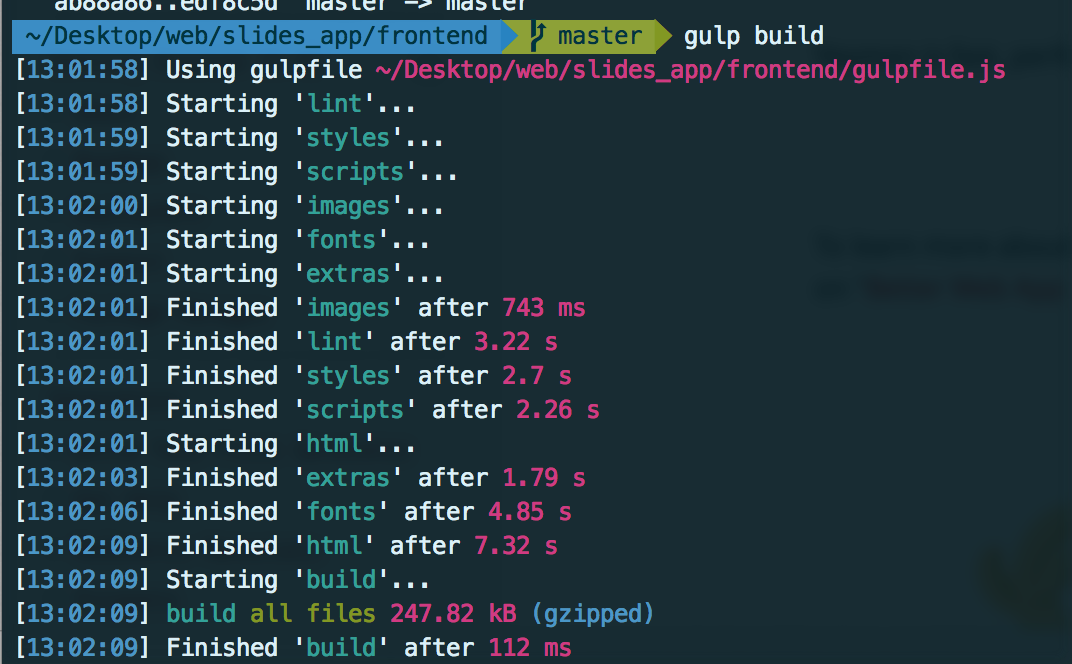
\includegraphics[width=.6\linewidth]{gulp_build.png}
  \caption{Frontend build using gulp}
\end{minipage}%
\begin{minipage}{.5\textwidth}
  \centering
  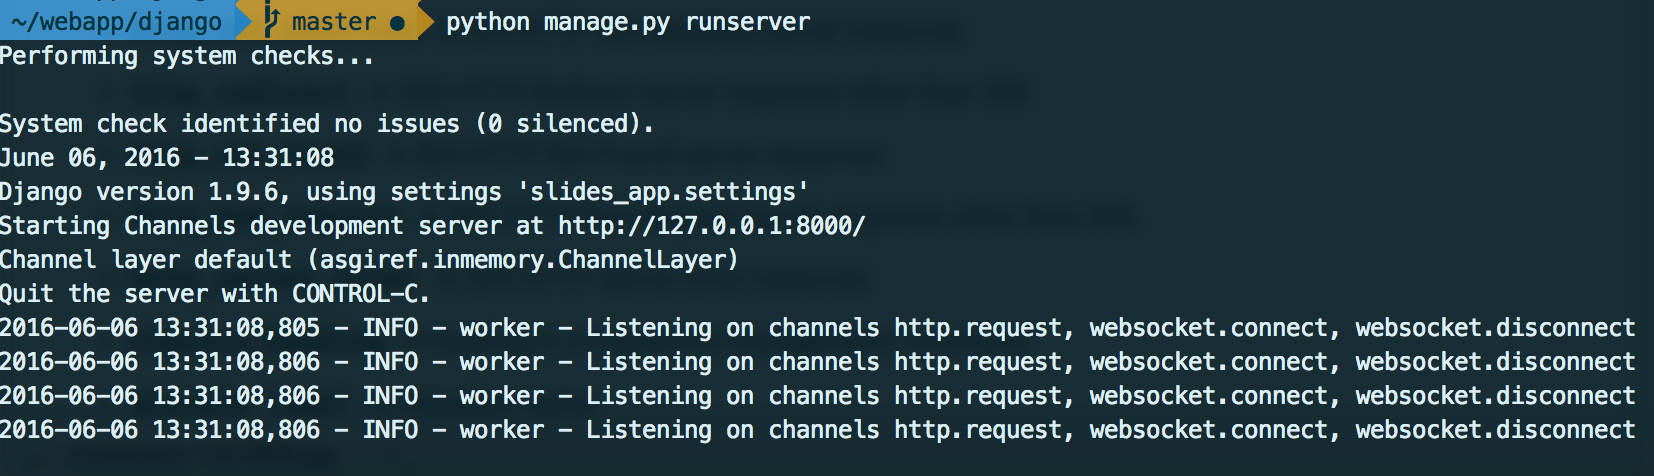
\includegraphics[width=.9\linewidth]{django_build.png}
  \caption{Running django backend server}
\end{minipage}%
\end{figure}

\end{document}
